\documentclass{article} 
\usepackage{amssymb,amsmath}
\usepackage{graphicx}
\usepackage{algorithmic}
\title{KE tableau prover, Design Decisions}
\author{Marc van Zee, 3714314} 
\begin{document} 
\maketitle
\section{Overview}
The global structure of the classes is represented in the flowchart below.\\*\\*
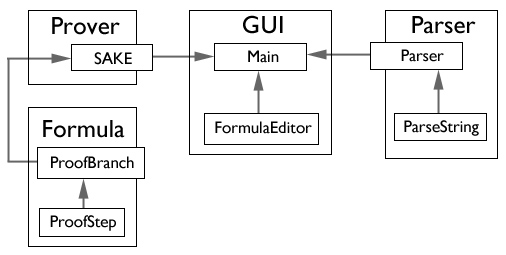
\includegraphics[height=180px]{flowchart.jpg}\\*\\*
An outgoing arrow from a class means that the class is being instantiated in the class where the arrow points at. As can be seen in the image, the overall structure consists of four packages that each cover a part of the tableau prover. A fifth package, $Lib$, is not included because it contains static methods and constants that are being used throughout the entire project.

I have chosen for this amount of classes because of simplicity. While I am sure that the actual prover could be written in two classes (or even one), I believe a more elaborate structure makes the project more insightful and easier to alter.

Having said this, I admit that the structure does not allow a lot of freedom regarding to the sort of logic used. I have chosen to use propositional logic; changing it to (for example) first order predicate logic requires significant changes in the $parser$, the $prover$ and, to a lesser extend, the $formula$ packages.

One might wonder why I have chosen to design a GUI, while the program could actually also work very well using the command line. For this I have two reasons:
\begin{itemize}
\item I believe that, as a student and in general, it is important to create work that is presentable. I believe that the current program is a lot more appealing and easier to use than a command line.
\item I have not found Java applications that show the working of a SAKE refuter using an applet. winKE does this, but it does not have web interface. My program could well be used as an example of the working of SAKE with regard to propositional logic for information databases such as wikipedia.
\end{itemize}

This is also a reason why I did not make use of first order logic. I wanted to design a program that functions well and is complete. \\\\I now will describe the different classes in the project, and the decisions made while designing them.
\newpage
\section{SAKE}
I will start off with the $SAKE$ class, since it is the class most relevant to the assignment that I made this program for. It can be generally described using the following algorithm, where $formula$ represents the formula to refute:\\\\
{\bf SAKE}, refutation algorithm

\begin{algorithmic}
\REPEAT
\IF{$formula$ contains contradiction}
\STATE{write "$X$" to $prooftree$}
\STATE{return $true$;}
\ENDIF
\STATE{try reductions in $formula$, save in $reductions$};
\STATE{write $formula$ and $reductions$ to $prooftree$};
\UNTIL{$reductions$ is $null$};
\STATE{try $DC$ on $formula$, save in $dc$;}
\IF{$dc$ is $null$}
\STATE{return $false$}
\ENDIF
\STATE{write dc messge to $prooftree$}
\STATE{$branch1$ = new {\bf SAKE}($formula$ + $dc$)};
\IF{$branch1$ is not provable}
\STATE{return $false$}
\ENDIF
\STATE{$branch2$ = new {\bf SAKE}($formula$ + $\neg dc$)};
\IF{$branch2$ is not provable}
\STATE{return $false$}
\ENDIF
\STATE{write $branch1$ and $branch2$ to $prooftree$}
\STATE{return $true$}
\end{algorithmic}
$\ $\\\\
{\bf Details of the algorithm}\\
The first thing the algorithm does is looking for a contradiction. This is the fastest way to close a branch since it does not require a prove step. Next, it will try to do all the reductions possible on the formula, in the following order:
\begin{itemize}
\item removeNegations(): looks for double negations;
\item removeDoubles(): remove double appearances of subformulas;
\item betaSubsumption();
\item etaReductions();
\item betaReductions();
\item alphaReductions();
\end{itemize}

When these reductions are no longer possible, DC is tried on the formula. It looks for the least complex sub-formula of a possible beta formula. If this does not succeed, a countermodel is printed. If DC succeeds, two branches are being created with the formula produced by DC added in one branch, and its negation in the other. The same process is repeated on each of the branches. The branchpoints at each DC step are being counted, so that it will be clear in the output at what point in branch the algorithm is.\\\\
{\bf Considerations}\\
As always in programming, one finds possibilities for improvement when finished. I personnaly would suggest the use of another class $Reductions$, that takes care of all the alpha, beta and eta reductions. This is because these reductions share the same structure, namely:\\
$formula1(+formula2) \rightarrow formula3(+formula4)$\\
Where $formula3$ and $formula4$ are always identical to $formula1$ or $formula2$, or a negated version of it. These restrictions could serve as arguments in a function call.

\section{Formula/Subformula}
A $Formula$ object is simply a collection of $Subformula$ objects. Therefore, it contains methods for operations on $Subformula$ objects. The reason why I did not simply use a collection of $Subformula$ objects without the $Formula$ class, is that in this way, the entire formula can be treated as an object, which makes it both more usable and insightful.

A $Subformula$ object consists of a literal, or two $Subformula$ objects and a connective. Also, it contains the number of negations over it.

\section{Parser/ParseString}
The parser instantiates a $ParseString$ object, which represents the string that is currently being parsed. The higher level commands are being given in the $Parse$ class, while $ParseString$ takes care of the more technical details.

It has the following restrictions considering the input:
\begin{itemize}
\item For propositions, one or more characters $[a-z],[A-Z],[0-9]$ are allowed, but note that all the characters will be converted to lowercase before parsing. This is to prevent the user from making typos;
\item The connectives are stored in the $Chars$ class, and can be changed before compiling;
\item Any number of parentheses, negations or whitespaces are allowed in the input formula;
\end{itemize}
As a result of its structure, the parser is right associative, which means that an input formula such as $p\Rightarrow q\wedge r$ will be interpreted as $p\Rightarrow (q\wedge r)$. This is because the parser searches the string for a connective at the lowest depth (with the minimal number of parentheses around it), and stores this position. If there happen to be two connectives at the lowest level, the last one will be saved (because it has been found last).

Although this right associativity works well for input formulas, I would not recommend to depend on it completely, since it is merely a result of the algorithm, and it has not been debugged enough.

\section{ProofBranch,ProofStep}
When all the branches of the proof close, meaning that they all lead to contradictions, the refutation can be turned into a proof. During every refutation in the $SAKE$ class, a $ProofBranch$ object is being created, which contains all the proof steps (indeed, saved as $ProofStep$ objects). Every time DC succeeds, the $ProofBranch$ object sets its $hasDC$ flag to $true$, and contains two branches that both are $ProofBranch$ objects again.

When asked to print the proof tree in the GUI, the $ProofBranch$ object will recursively print out all steps, starting with its branches (only if its $hasDC$ flag holds, of course). Then it will print its proof steps, from end to start. Before printing the proof, the $ProofBranch$ object at the top (the one instantiated in $SAKE$) has to be fed with a starting number (I have used 1). It will then number all the proof steps, which will make the final proof better to read.

\section{Chars}
This class contains all the constant characters that are being used throughout the program, which are all of the connectives, the negation character and the parentheses. These can be changed here.

\section{FormulaComp}
This class contains several static methods that operate on two $Subformula$ objects which are given as arguments. They are in a seperate class because they do not belong to any object; they are merely methods for calculation.
\\\\
For a more details description on the methods, please refer to the JavaDoc and the source code.
\end{document}